\documentclass[11pt]{jsarticle}
\usepackage[dvipdfmx]{graphicx}
\title{名合のここがかわいい!}
\author{匿名希望のバレー部員カラオケ要員}
\date{\today}
\begin{document}
\maketitle

\section{みんな友達!}
\subsection{坂内君は男友達であって異性じゃない}
\subsection{稲本君は友達でもない}
\subsection{サカキダって?}
\section{番外編}
\subsection{間違えちゃったな、合}
\section{最後に}


\newpage
\part{坂内君は男友達であって異性じゃない}
\,2019年の(確か)明大明治で出た言葉。
\,稲本の告げ口により坂内が名合のことを「女友達」としてみていることがばれ、
\,名合が対抗して放った言葉である。このイベントでは名合との好感度が50以上ないと
\,即死イベントとなるので注意が必要。よかったね。坂内君。
\newpage
\part{稲本君は友達でもない}
\,泣きそう。
\newpage
\part{サカキダって?}
\,サカキダという謎の多い人物について。部活中にだらけているとどこからか
\,「もう部活やめる...」という声が聞こえてくる。聞き覚えのある声だが
\,筆者も覚えていない。あれ、昨日のカラオケ坂内と俺と...あと一人。
\,あの生真面目な...まあいいや。
\newpage
\part{番外編:間違えちゃった合part1}
\,名合お茶目ポイントを図1.2.3に示す.

\begin{figure}[htbp]
 \begin{minipage}{0.33\hsize}
  \begin{center}
   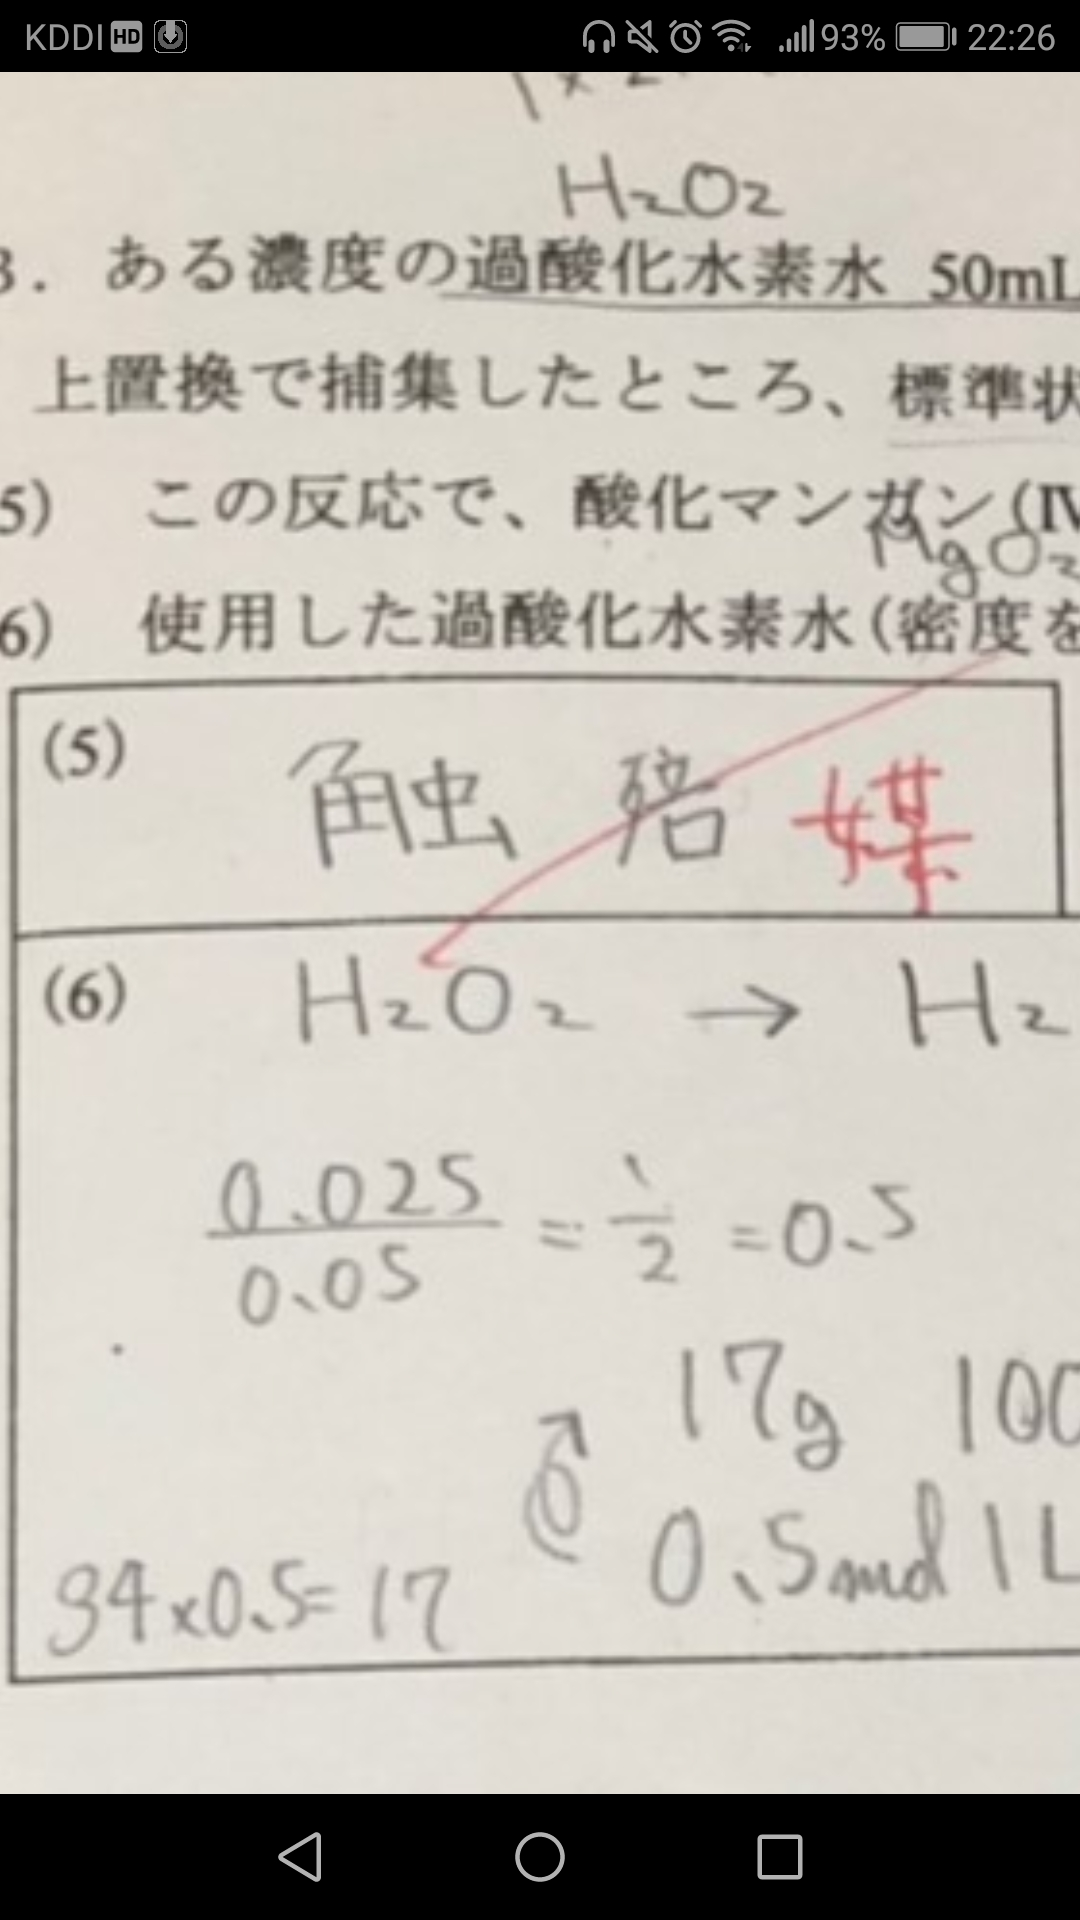
\includegraphics[scale=0.1]{pic.jpg}
  \end{center}
  \caption{一つめの図}
  \label{fig:one}
 \end{minipage}
 \begin{minipage}{0.33\hsize}
 \begin{center}
  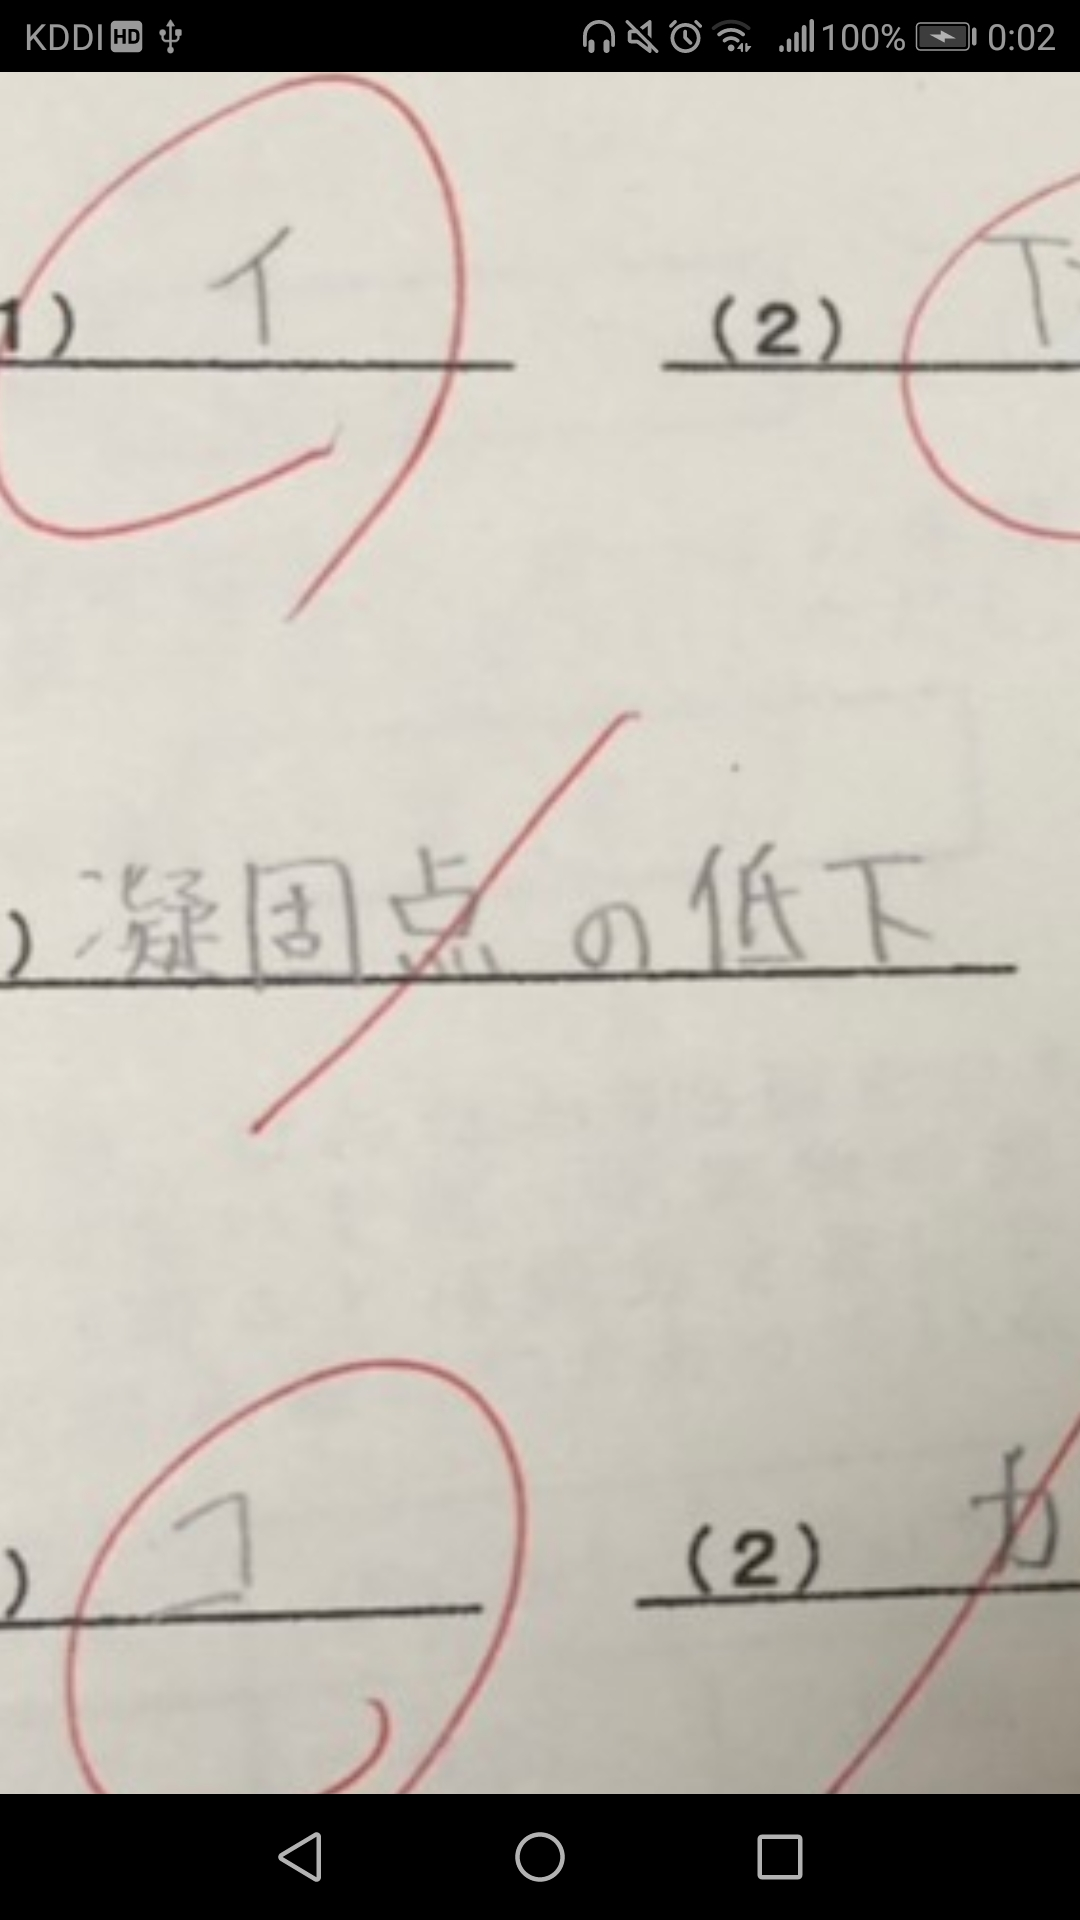
\includegraphics[scale=0.1]{pic2.jpg}
 \end{center}
  \caption{二つめの図}
  \label{fig:two}
 \end{minipage}
 \begin{minipage}{0.33\hsize}
 \begin{center}
  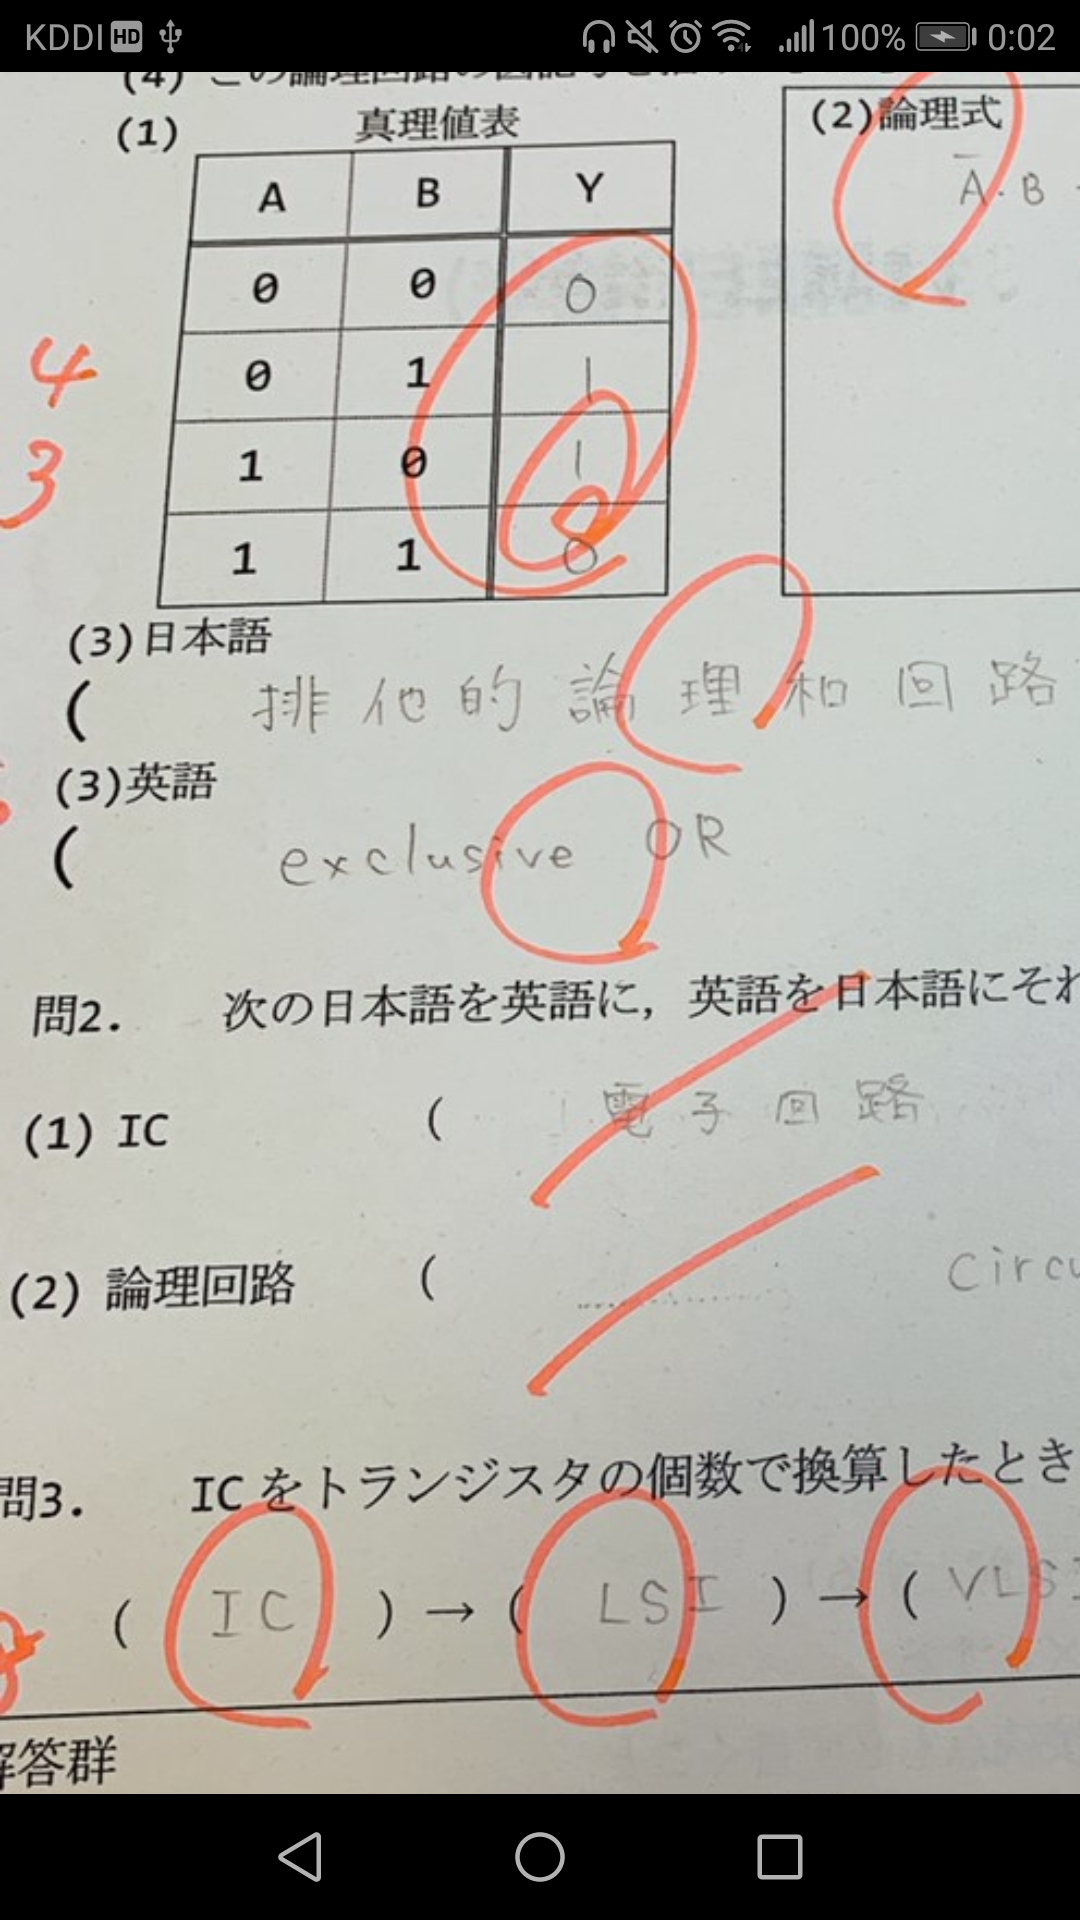
\includegraphics[scale=0.1]{pic3.jpg}
 \end{center}
  \caption{三つめの図}
  \label{fig:three}
 \end{minipage}
\end{figure}

\begin{thebibliography}{数字}
  \bibitem{かぎそ過去問} 名合が送ったかぎそ過去問より・一年前の名合
\end{thebibliography}
\newpage
\part{最後に}
\,このPDFの著作権は著者に依存します。
\,間違っても名合に見せたりしないでください。
\,ふりじゃないです。



\end{document}
